%%%%%%%%%%%%%%%%%%%%%%%%%%%%%%%%%%%%%%%%%
% Beamer Presentation
% LaTeX Template
% Version 1.0 (10/11/12)
%
% This template has been downloaded from:
% http://www.LaTeXTemplates.com
%
% License:
% CC BY-NC-SA 3.0 (http://creativecommons.org/licenses/by-nc-sa/3.0/)
%
%%%%%%%%%%%%%%%%%%%%%%%%%%%%%%%%%%%%%%%%%

%----------------------------------------------------------------------------------------
%	PACKAGES AND THEMES
%----------------------------------------------------------------------------------------

\documentclass{beamer}

\mode<presentation> {

% The Beamer class comes with a number of default slide themes
% which change the colors and layouts of slides. Below this is a list
% of all the themes, uncomment each in turn to see what they look like.

%\usetheme{default}
%\usetheme{AnnArbor}
%\usetheme{Antibes}
%\usetheme{Bergen}
%\usetheme{Berkeley}
%\usetheme{Berlin}
%\usetheme{Boadilla}
%\usetheme{CambridgeUS}
%\usetheme{Copenhagen}
%\usetheme{Darmstadt}
%\usetheme{Dresden}
%\usetheme{Frankfurt}
%\usetheme{Goettingen}
%\usetheme{Hannover}
%\usetheme{Ilmenau}
%\usetheme{JuanLesPins}
%\usetheme{Luebeck}
\usetheme{Madrid}
%\usetheme{Malmoe}
%\usetheme{Marburg}
%\usetheme{Montpellier}
%\usetheme{PaloAlto}
%\usetheme{Pittsburgh}
%\usetheme{Rochester}
%\usetheme{Singapore}
%\usetheme{Szeged}
%\usetheme{Warsaw}

% As well as themes, the Beamer class has a number of color themes
% for any slide theme. Uncomment each of these in turn to see how it
% changes the colors of your current slide theme.

%\usecolortheme{albatross}
%\usecolortheme{beaver}
%\usecolortheme{beetle}
%\usecolortheme{crane}
%\usecolortheme{dolphin}
%\usecolortheme{dove}
%\usecolortheme{fly}
%\usecolortheme{lily}
%\usecolortheme{orchid}
%\usecolortheme{rose}
%\usecolortheme{seagull}
%\usecolortheme{seahorse}
%\usecolortheme{whale}
%\usecolortheme{wolverine}

%\setbeamertemplate{footline} % To remove the footer line in all slides uncomment this line
%\setbeamertemplate{footline}[page number] % To replace the footer line in all slides with a simple slide count uncomment this line

%\setbeamertemplate{navigation symbols}{} % To remove the navigation symbols from the bottom of all slides uncomment this line
}

\usepackage{graphicx} % Allows including images
\usepackage{booktabs} % Allows the use of \toprule, \midrule and \bottomrule in tables
\usepackage{listings}
\usepackage{amsmath}
\usepackage{algpseudocode,algorithm,algorithmicx}

\lstdefinestyle{customjava}{
  breaklines=true,
  frame=L,
  xleftmargin=\parindent,
  language=Java,
  showstringspaces=false,
  basicstyle=\footnotesize\ttfamily,
  keywordstyle=\bfseries\color{green!40!black},
  commentstyle=\itshape\color{gray!40!black},
  identifierstyle=\color{blue},
  stringstyle=\color{orange},
}

%----------------------------------------------------------------------------------------
%	TITLE PAGE
%----------------------------------------------------------------------------------------

\title[Upper Layers]{Upper Layers} % The short title appears at the bottom of every slide, the full title is only on the title page

\author{Jonathan Windle} % Your name
\institute[UEA] % Your institution as it will appear on the bottom of every slide, may be shorthand to save space
{
University of East Anglia \\ % Your institution for the title page
\medskip
\textit{J.Windle@uea.ac.uk} % Your email address
}
\date{\today} % Date, can be changed to a custom date

\begin{document}

\begin{frame}
\titlepage % Print the title page as the first slide
\end{frame}

\begin{frame}[allowframebreaks]
\frametitle{Overview} % Table of contents slide, comment this block out to remove it
\tableofcontents % Throughout your presentation, if you choose to use \section{} and \subsection{} commands, these will automatically be printed on this slide as an overview of your presentation
\end{frame}

%------------------------------------------------------------------
\section{Intro}
\begin{frame}
\frametitle{Intro}
\begin{itemize}
\item Contains:
\begin{itemize}
\item Application Layer (layer 7)
\item Presentation Layer (layer 6)
\item Session Layer (layer 5)
\end{itemize}
\end{itemize}
\end{frame}
%-------------------------------------------------------------------
\section{Application Layer - 7}
\begin{frame}
\frametitle{Description}
\begin{itemize}
\item Significantly different from other layers
\item Lower layers concerned with reliably communicating data from one process/machine to another.
\item Application layer concerned with what to do with data once it arrives.
\item Has a set of utilities:
\begin{itemize}
\item {\color{red} Specific Application Service Elements (SASE)} - FTAM, MHS, DS, VT
\item {\color{green} Common Application Service Elements (CASE)} - provide access to Presentation layer, plus {\color{purple}Concurrency Commitment and Recovery (CCR)}.
\end{itemize}
\end{itemize}
\end{frame}
%----------------------------------------------------------------
\subsection{Specific Application Service Elements - SASE}
\begin{frame}
\frametitle{Specific Application Service Elements - SASE}
\begin{itemize}
\item Basically abstractions for commonly used high-level network operations (procedure/interrupt libraries).
\item {\color{red} FTAM - File Transfer Access \& Management} implements a virtual filestore.
\item {\color{green} MHS - Message Handling Service} for E-Mail applications.
\item {\color{purple} DS - Directory Service} allow network services to be known by symbolic names. Implements a mapping of $names \rightarrow network \ ids \ (TSAP's)$.
\item It allows operations to add/change/delete entrues so that processes can advertise ttheir existence, be closed down etc.
\end{itemize}
\end{frame}
%--------------------------------------------------------------------
\subsection{Common Application Service Elements (CASE)}
\begin{frame}
\frametitle{Common Application Service Elements (CASE)}
\begin{itemize}
\item CASEs are primitives to give access to {\color{red} Presentation Layer} equivalents.
\item Commitment, Concurrency \& Recovery (CCR).
\item CCR implements fool-proof coordination of mult-message operations to difference computers even under repeated host crashes.
\item Implemented by supporting {\color{green} atomic actions} (either fail or completelet succees in their entirety).
\item Requires Stable storage (i.e. disk storage) to hold state information and a 2 stage prepare then commit.
\end{itemize}
\end{frame}
%-----------------------------------------------------------------
\section{Presentation Layer - 6}
\begin{frame}
\frametitle{Description}
\begin{itemize}
\item Main concerns:
\begin{itemize}
\item Access to the session layer
\item Representation transformations
\end{itemize}
\item It's concerned with preserving the meaning of information sent over the network.
\item It may represent the data (encode) in various ways, but the receiver side will convert it back into its original meaning.
\end{itemize}
\end{frame}
%---------------------------------------------------------------
\subsection{Issues}
\begin{frame}
\frametitle{Issues}
\begin{itemize}
\item \textbf{ Data format:} Convert data structures used on a machine (floats, ints, characters etc) into byte sequence. {\color{red} Peers} agree on the format before exchanging. E.g. How many bytes to represent an integer etc.
\item \textbf{Compression:} Reducing the number of bits required to transmit infomation.
\item \textbf{Encryption/Privacy:} Encrypting data so that only authorised participants can read it. {\color{green} Authentication} - verifying that remote party is really who they claim to be.
\end{itemize}
\end{frame}
%-----------------------------------------------------------------
\subsection{Source coding standards}
\begin{frame}
\frametitle{Source coding standards}
\begin{itemize}
\small
\item Standards for encoding source data are termed {\color{green} source coding standards}.
\item Have two main functions:
\begin{itemize}
\item Ensure common format which manufacturers can adopt to ensure compatibility of devices.
\item Compression of the original source signal such that a good representation can be made using a smaller number of bits (for transmission and storage).
\end{itemize}
\item Can be {\color{red} lossless} or {\color{purple} lossy} depending on media type. Images and audio can tolerate {\color{purple} lossy} compression whereas text and binaries cannot.
\item To maintain a high quality with a much reduced bit rate, the computational complexity is a real disadvantage.
\item Can use a model to compress effectively, for example speech will compress by removing sounds outside of a {\color{magenta} frequency resolution} (Ear has a lower frequency resolution at higher frequencies) and {\color{blue}masking}(Strong signals mask out neighbouring signals).
\item To deal with variable signal strengths, the bit rates can vary too, due to more error checking needed at poorer signal strengths.
\end{itemize}
\end{frame}
%-----------------------------------------------------------------
\subsection{Audio Coding standards}
\begin{frame}
\frametitle{Audio Coding standards}
\begin{itemize}
\item {\color{red} Bit rate} (number of bits needed to represent one second of data) is given by:\\
{\scriptsize
$Bitrate = number \ of \ samples \ per \ second \ \times number \ of \ bits \ per \ sample \ \times \ number \ of \ channels \ (mono/stereo)$}
\item {\color{green} Total amount of data} can be calculated by:\\
{\scriptsize
$Total \ amount = \ number \ of \ bits \ per \ second \ \times \ number \ of \ seconds$}
\item {\color{purple}Download time} is calculated by:\\
{\scriptsize 
$Time \ to \ download = \frac{Size \ of \ file}{data \ rate}$}
\item To download faster, compress more or increase data rate (throughput).
\end{itemize}
\end{frame}

%-----------------------------------------------------------------------------
\subsection{Image Coding Standards}
\begin{frame}
\frametitle{Image Coding Standards}
\begin{itemize}
\item Black and white images only need one bit per pixel and therefore an entire image is:\\
$Size = pixels \times 1$
\item Colour images require 24 bits per pixel (8 red, 8 green, 8 blue) and therefore:\\
$Size = pixels \times 24$
\end{itemize}
\end{frame}
%-------------------------------------------------------------------
\section{Session Layer - 5}
\begin{frame}
\begin{itemize}
\frametitle{Descriptions}
\item Session layer and presentation layer add services to that offered by the transport layer which may be useful to the application layer.
\item Avoids the application layer having to implement these itself.
\item Some models (TCP/IP) the functionality of session and presentation layers is put in application and transport layers.
\item This is the \"Thinnest" layer in the OSI reference model.
\item Main functions:
\begin{itemize}
\item Session connection establishment and release.
\item Synchronisation points
\item Dialogue interruption and resumption.
\end{itemize}
\end{itemize}
\end{frame}
%--------------------------------------------------------------
\subsection{Connection establishment}
\begin{frame}
\frametitle{Connection establishment}
\begin{itemize}
\item Transport layer connections accept session layer connections, termination requires orderly set up and release (both sides must agree) - 3-way handshake.
\item Opening can be denied. Similar process for release - can be denied if further message needs to be exchanged.
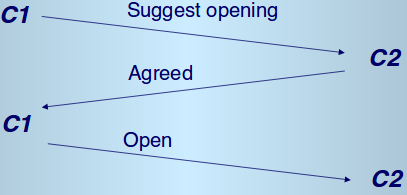
\includegraphics[scale=0.4]{sess.png}
\end{itemize}
\end{frame}
%-----------------------------------------------------------------
\subsection{Synchronization}
\begin{frame}
\frametitle{Synchronization}
\begin{itemize}
\item Points within a dialogue for recovery from agreed points if machine or network fails.
\item Transfers grouped into {\color{red}activities} and {\color{green}dialogues}.
\item {\color{red}Activities} and {\color{green}dialogues} can be structured as sequences of message exchanges punctuated by synchronization points.
\item Points have to be acknowledged and allow for reversion to the last sync point.
\end{itemize}
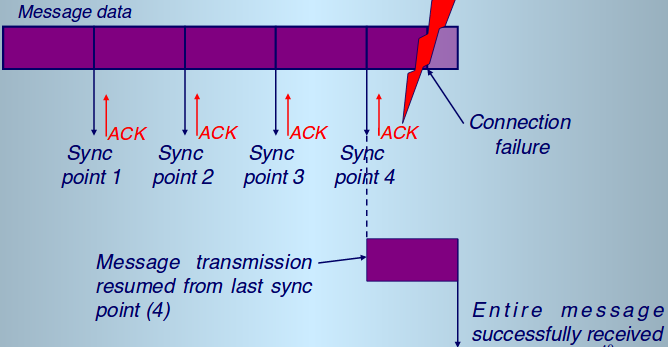
\includegraphics[scale=0.3]{synch.png}
\end{frame}
%-----------------------------------------------------------
\section{Summary}
\begin{frame}
\frametitle{Summary}
\begin{itemize}
\item Examined the functions of the top three layers of the OSI reference model (and TCP/IP model)
\item \textbf{Application layer:} Provision of functionality and for multi-party atomic actions
\item \textbf{Presentation layer:} Provision for computer independant transfer syntax, compression and encryption.
\item \textbf{Session layer:} Establishing session between machines, synchronization and dialogue control.
\item Applications typiclly require some of these facilities.
\item TCP/IP combines these layers into one layer.
\end{itemize}
\end{frame}

%-----------------------------------------------------------------
\begin{frame} 
\Huge{\centerline{The End}}
\end{frame}
\end{document}